\customHeader{1}{Tokenization and Embeddings}
\label{02_tokenization_and_embeddings}

Most \gls{nlp} tasks for text start with a corpus of documents. The documents may have been manually collected by humans; automatically collected, for example, using web scrapping tools, generating text from templates, or, most recently, sampling outputs from \gls{ai} tools like GPT-3 \myparencite{wang-etal-2021-want-reduce} and ChatGPT \myparencite{huang2023chatgpt}; or constructed using a mixture of human and automatic input.

Considering the ever-changing nature of natural language, the initial phase in \textclassification{} involves defining the system's Vocabulary. \emph{\tokenization{}} refers to the act of segmenting text into smaller units, known as \emph{tokens}. As a first approach, one may use the intuitive idea of \emph{word} for tokens, in languages with a morphosyntax similar to English (Figure \ref{fig:naive_tokenization}). The collection of unique tokens derived from a text corpus forms the Vocabulary.

\begin{figure}
    \centering
    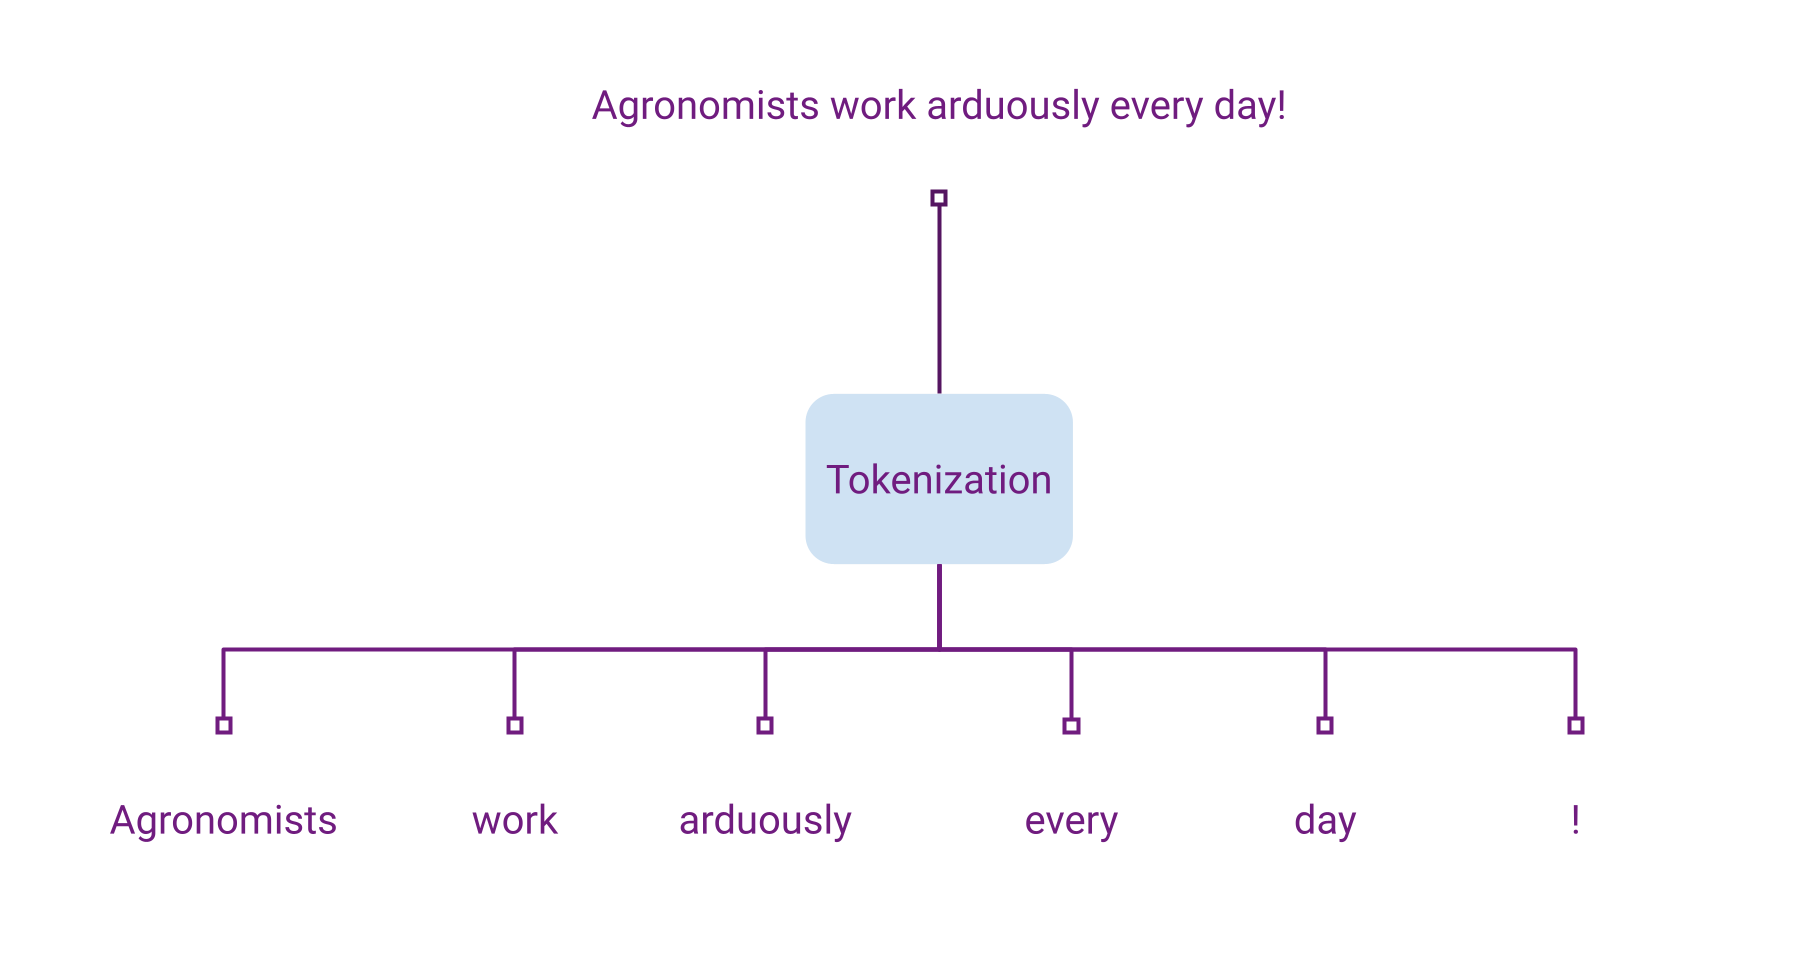
\includegraphics[width=0.75\textwidth]{Figures/02/01_Naive_Tokenization.png}
    \caption{Naive tokenization}
    \label{fig:naive_tokenization}
\end{figure}

However, naive word tokenization\footnote{Another simple tokenization technique is \emph{character-level tokenization}, where text is simply divided into individual characters. This tokenization technique falls outside the scope of this work.} can lead to challenges with out-of-vocabulary (OOV) words when presented with new data. 
A more modern tokenization approach involves using \emph{subword units}. This strategy addresses OOV words by breaking words down into smaller segments. In English, for instance, one might consider prefixes and suffixes as subwords (like \texttt{pre-}, \texttt{-ing}, \texttt{-ed}, and so on), enhancing the \gls{nlp} system's ability to understand morphology. Nevertheless, instead of manually defining rules to divide words into subwords, there are two widely-used algorithms based on frequency to create such tokenizers:


\begin{itemize}
    \item \emph{\gls{bpe}} \myparencite{sennrich2015neural} builds a vocabulary by iteratively merging the most frequent pair of characters or character sequences in a given text corpus. It starts with a character-level vocabulary and merges the most frequent pair of tokens until a desired vocabulary size is reached.
    \item \emph{\gls{wp}} \myparencite{wu2016google} begins by creating a vocabulary that consists of all the characters found in the training data. It then proceeds to learn a specific number of merge rules. Unlike \gls{bpe}, \wordpiece{} Tokenization selects symbol pairs that maximize their frequency relative to its constituent symbols, rather than choosing the most frequent symbol pair.
\end{itemize}

Typically, these algorithms result in different tokenizations for the same text, leading to different vocabularies. Figure \ref{fig:02_tokenizer_comparison} displays a sample output from the \gls{wp} method in \mytextcite{BERT_paper} and the \gls{bpe} method in \mytextcite{roberta} for English content.


\begin{figure}
    \centering
    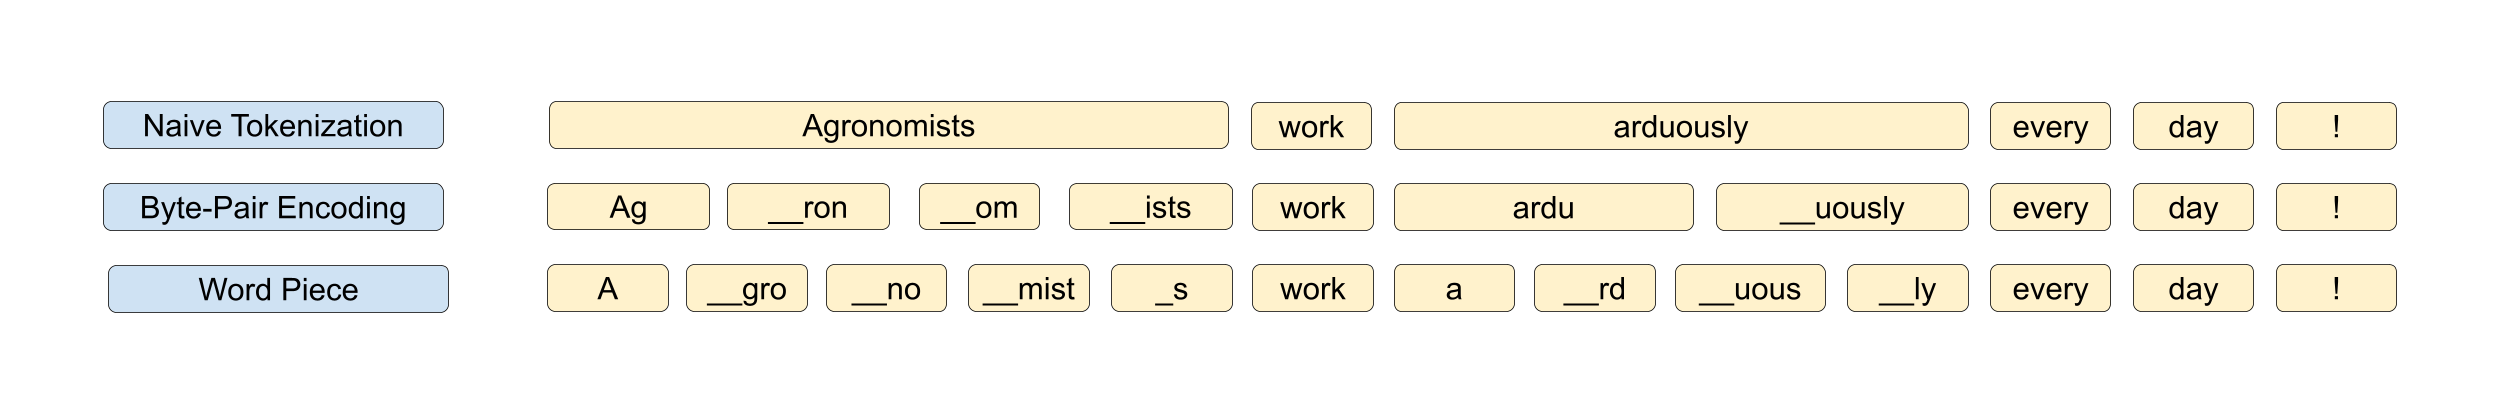
\includegraphics[width=\textwidth]{Figures/02/02_Tokenizer_comparison.png}
    \caption{Different tokenization approaches:\\ naive, \bpe{}, and \wordpiece{}}
    \label{fig:02_tokenizer_comparison}
\end{figure}

Even though there are \textclassification{} approaches which only consider the distribution of tokens in a corpus, like \emph{Naive Bayes Classification} \myparencite{statistical_nlp_naive_bayes}, recent breakthroughs in \gls{nlp} have been enabled by \emph{text embeddings}, which are vector representations of text in high-dimensional space. 

\putInBox{
Embeddings are intended to capture the semantic relationships between texts, allowing computational models to understand and manipulate textual data.  
Typically, embeddings serve as \emph{input features} for textual data, which are then fed into \gls{ml} algorithms (Figure \ref{fig:02_embeddings_for_training_classification}).
}

\emph{Word embeddings} are a type of text embedding that assign a vector representation to each token in a text.
Within \textclassification{}, while word embeddings are prevalent, Document Classification especially benefits from \emph{Document embeddings}. These embeddings provide a unique vector representation for an entire document, enabling a holistic understanding and categorization of texts based on their full content and context. 
Essentially, text embeddings ensure that texts with analogous meanings are closely aligned, while those with divergent meanings are distinctly separated (Figure \ref{fig:word_and_document_embeddings}).


\begin{figure}
    \centering
    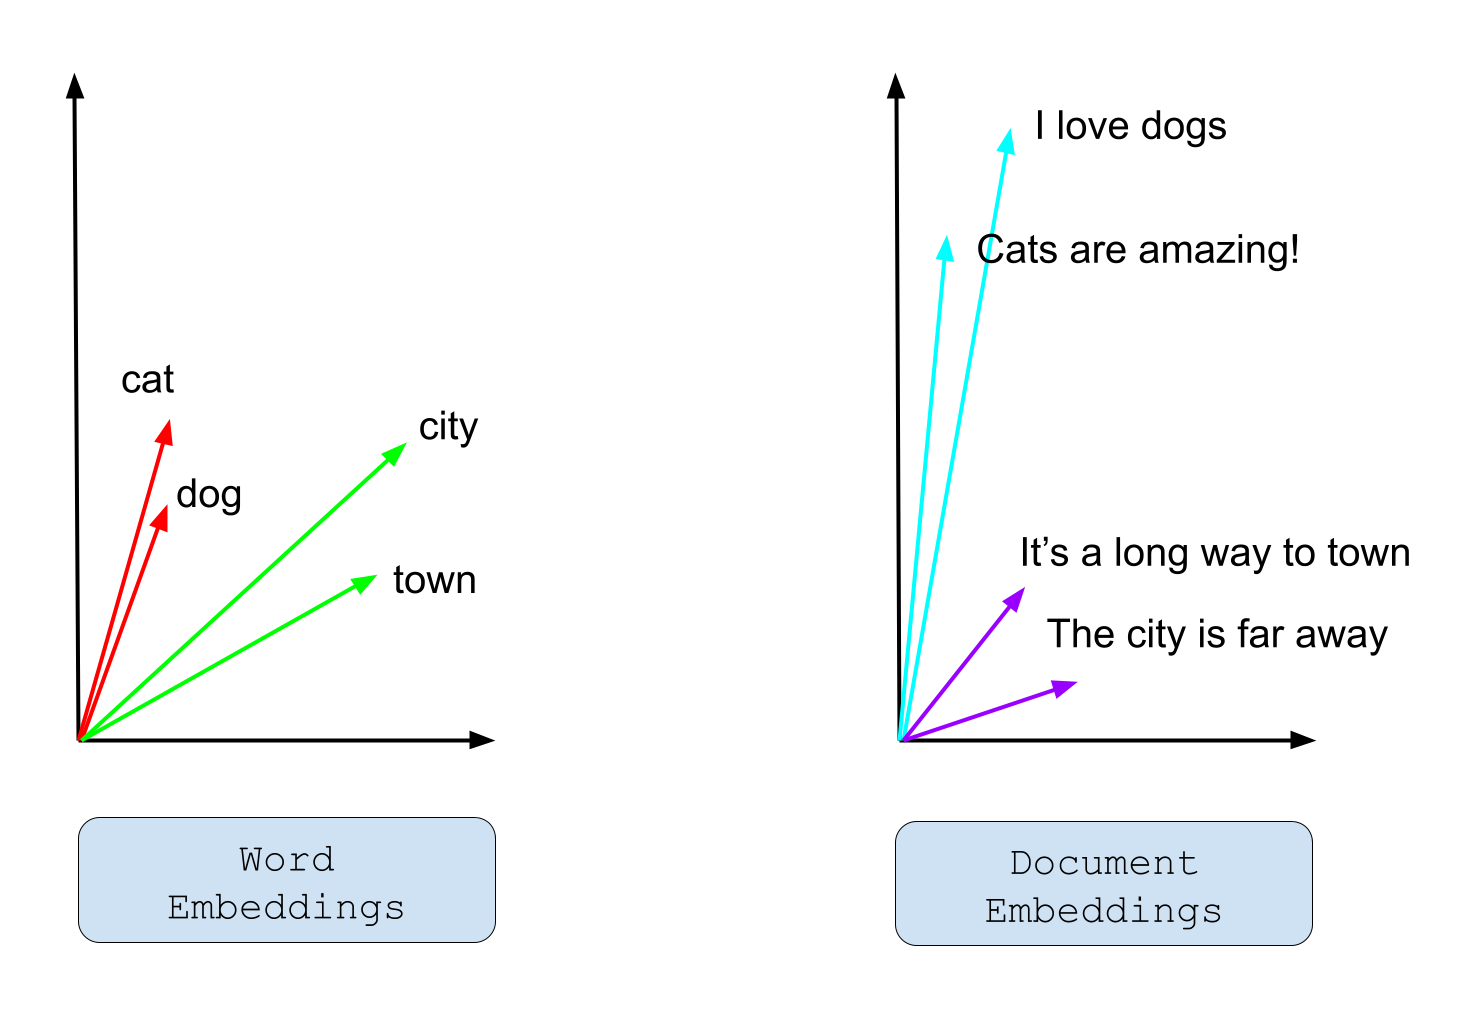
\includegraphics[width=0.5\textwidth]{Figures/02/02_embeddings.png}
    \caption{Word and Document embeddings}
    \label{fig:word_and_document_embeddings}
\end{figure}

\begin{figure}
    \centering
    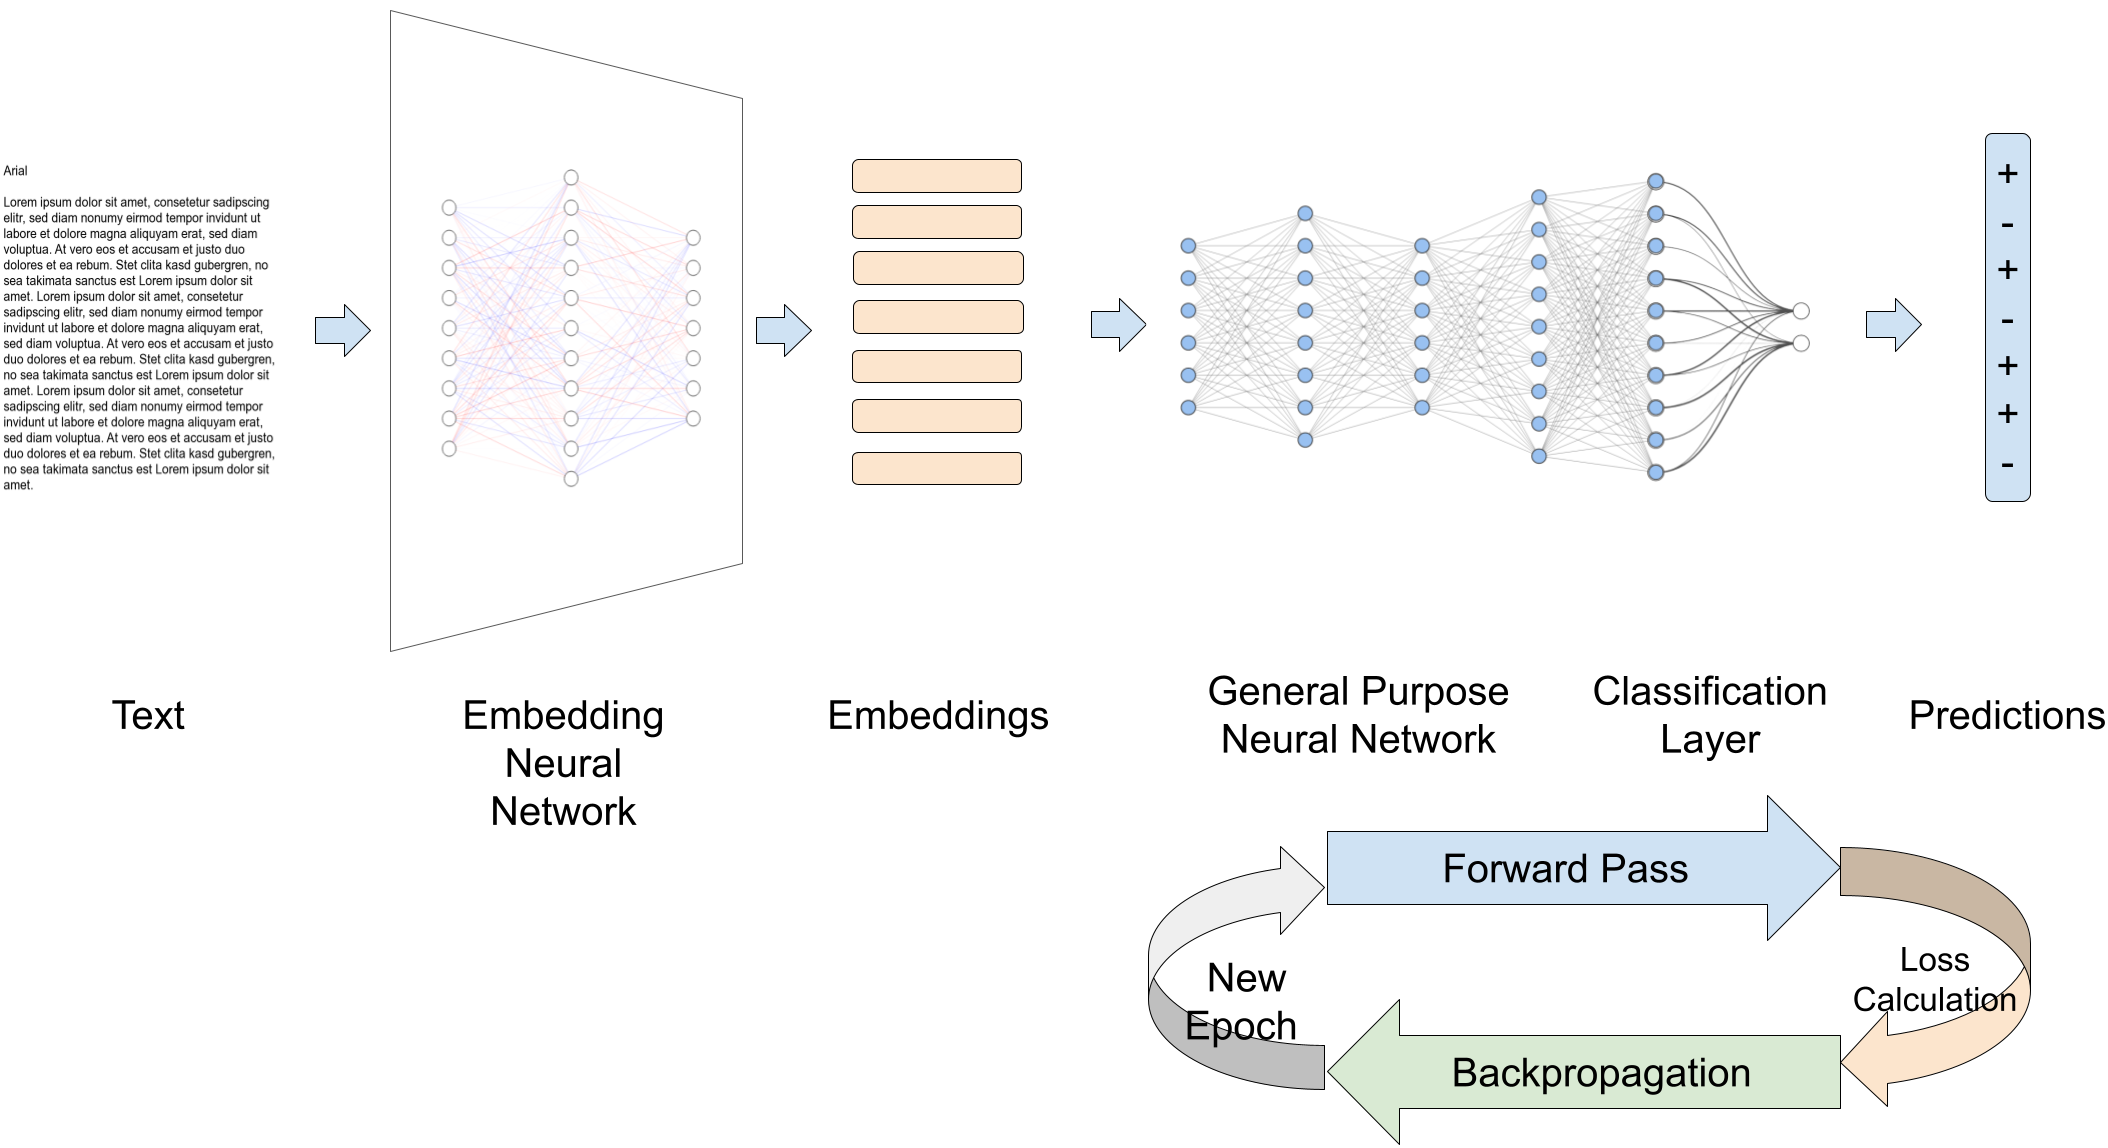
\includegraphics[width=\textwidth]{Figures/02/02_nns_for_nlp.png}
    \caption{Using Embeddings to train Neural Networks for Classification}
    \label{fig:02_embeddings_for_training_classification}
\end{figure}

Text embeddings have undergone significant evolution over the years, with several techniques and models contributing to their development. We present a brief overview of the key milestones in the evolution of word embeddings:

\begin{itemize}
    \item Early approaches focused on frequency-based representations, such as Bag-of-Words (BOW) one-hot encoding\footnote{A one-hot vector has all its components null, except one which has value one} and term frequency-inverse document frequency (TF-IDF). These methods assigned weights or binary values to words based on their occurrence in the corpus, without capturing semantic relationships.
    \item \emph{Word2Vec} \myparencite{mikolov2013linguistic} popularized the concept of word embeddings trained using unsupervised learning. These models utilized shallow neural networks to learn word embeddings by predicting neighboring words or contexts. 
    \item \emph{GloVe} embeddings \myparencite{pennington-etal-2014-glove}  were trained on word co-occurrence statistics from a large corpus. It leveraged both global word co-occurrence information and local context windows to create meaningful vector representations.
    \item \gls{rnn} architectures, such as GRU (Gated Recurrent Unit), LSTM (Long Short-Term Memory),  and Bi-LSTM (bidirectional LSTM), provided a breakthrough in capturing sequential dependencies and long-term dependencies within sentences, for example with \emph{InferSent} document embeddings \myparencite{infersent_bilstm}. By processing sentences sequentially, \gls{rnn}s generated fixed-dimensional vector representations at the sentence level. However, they faced challenges with long-term dependencies and were computationally expensive for longer sentences.
    
    \item  Contextualized word embeddings introduced the idea of generating word representations that varied depending on the context in which they appeared. Models like \emph{ElMo} (Embeddings from Language Models) \myparencite{elmo} and OpenAI's GPT (Generative Pre-trained Transformer) \myparencite{gpt} employed deep contextualized models and transformers to produce dynamic word embeddings.
    \item Transformer models, including Google's \gls{bert} (Bidirectional Encoder Representations from Transformers) 
    \myparencite{BERT_paper}, OpenAI's GPT-2 \myparencite{gpt2} and GPT-3 \myparencite{gpt3}, revolutionized the field by leveraging attention mechanisms and large-scale pre-training. These models introduced contextualized word embeddings on a larger scale and achieved state-of-the-art performance across various NLP tasks. %The \BERT{} family of models has gained significant popularity due to its ability to efficiently generate contextualized embeddings for both individual tokens and entire documents at a low cost. Due to this factor, they will serve as primary tools in this project.
\end{itemize}


In this work, our primary focus is on employing the \gls{bert} family of models for \textclassification{}. The details of these models will be explored in the next section.
